\documentclass[11pt,journal]{IEEEtran}
\usepackage{amsmath}
\usepackage{graphicx}
\usepackage{listings}

\graphicspath{{./}}

\title{Emotion Recogniser}

\author{Tianqi (Carl) Liu, ~\IEEEmembership{z5019791} \\
        Han Zhang Zeng, ~\IEEEmembership{z1234567}}

\begin{document}
\maketitle
\begin{abstract}
    This is a report on the emotion recognizer project for comp9517 at UNSW. the report includes our goal, reference survey, problem decomposition, detailed specification, design, test and justification, group contribution and conclusion.
\end{abstract}

\section{Introduction}
  The goal of the project is to able to recognize human emotion on real time live stream to a degree of accuracy, at the start of the project we set the benchmark to around $70\%$ because for most current object recognition algorithm an accuracy of $70\%$ can be achieved (we will discuss this later in the test and design parts). There are 4 emotions that we are concerned with:

  \begin{enumerate}
    \item \textit{neutral}
    \item \textit{happy}
    \item \textit{angry}
    \item \textit{sadness}
  \end{enumerate}

  \textbf{other}: when the recognizer is not sure we consider the emotion to be some other emotion\\\\

  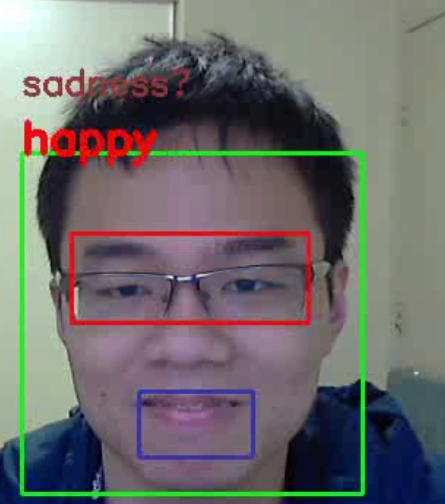
\includegraphics[width=0.4\textwidth]{01.png}

  For the final product, as shown in the photo, The face will be framed telling us which components are used for emotion recognition. There are 2 emotions displayed, the larger text on top of the face frame (Green) is the best estimation of the current emotion, the darker red text is the 2nd best predication.

\section{Problem Decomposition}
  The project consists of two major components:
  \begin{enumerate}
    \item \textbf{\textit{Face Extraction}}
    \item \textbf{\textit{Emotion Recognition}}
  \end{enumerate}

  \subsection{Face Extraction}
    In order to perform the emotion recoginition algorithm, we need to extract the face from the image. We decided to use the fisherface recognizer which requires the input image to be of fixed size (detailed explaination will be in survey section) therefore it is essential that we first extract the face.

    We chose the Haar Cascade algorithm for facial extraction because it is a really fast algorithm while maintaining a relatively high accuracy. Speed is very important for our application because during live stream, we want the algorithm to spend as little time as possible on the computation or else the stream will lag and the result will be unfavorable. Accuracy is not as important as speed in this context. When it comes to live stream, at every $\frac{1}{60}$ second, a new frame will be captured and computed, it is barely noticeable that one or two frames were not captured during a single second.


  \subsection{Emotion Recognition}
    The emotion recognition phase can be furthur classified into 2 parts.

    \begin{enumerate}
      \item \textbf{\textit{Training}}
      \item \textbf{\textit{Prediction}}
    \end{enumerate}

    In order to perform real time recognition we need fast algorithms, the best way to achieve this is to use a trained recognizer. The most common recognizers for the face are Haar Cascade Recognizer, Fisherface and Eigenface (details of each recognizer will be in survey sections)

    \subsection{Training}
      For the training process, we require large amount of data. We found a frontal face database from Cohn Kanade which contains $6000$ images on 7 emotions.

      \begin{enumerate}
        \item \textit{nuetral}
        \item \textit{contempt}
        \item \textit{disgust}
        \item \textit{fear}
        \item \textit{happy}
        \item \textit{sadness}
        \item \textit{surprise}
      \end{enumerate}

      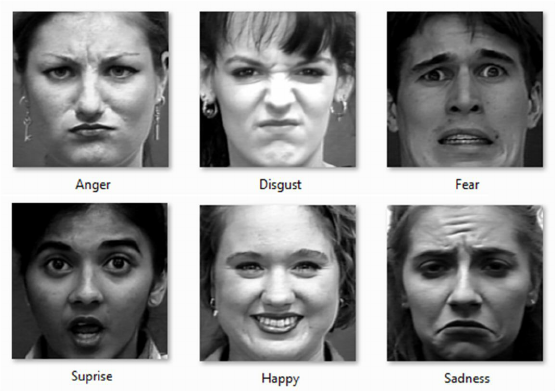
\includegraphics[width=0.4\textwidth]{02.png}
      \center{\textit{sample images}}

      We wrote a python code which classifies the emotions to folders named as the emotion, so in the happy folder contains all images that are happy

      
\includegraphics[width=0.4\textwidth]{03.png}
      \center{\textit{folder layout}}

      We train the recognizer by extracting the images from each of the folder, detailed explanation will be in algorithm design section.

    \subsection{Prediction}
      For the prediction phase, we extract the face using Haar Cascade then pass it into the recognizer, the recognizer will output a specific value that corresponds to one of the emotions. The emotion will be displayed on the screen above the head frame.

\end{document}
